\documentclass[border=4pt]{standalone}
\usepackage{tikz}
\usetikzlibrary{arrows.meta,decorations.markings}

\definecolor{orangeText}{HTML}{E3A063}
\definecolor{orangeDim}{HTML}{A87A4E}
\begin{document}
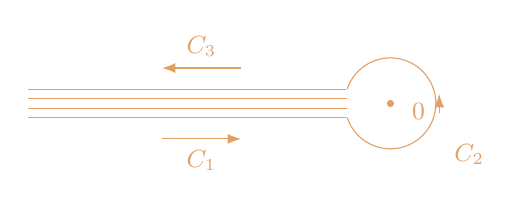
\begin{tikzpicture}[color=orangeText, >=Latex]

    \def\rc{0.55}
    \def\e{0.06}
    \tikzset{mid/.style={postaction={decorate,decoration={markings,
        mark=at position 0.5 with {\arrow{Latex}}}}}}

    % branch cut: two doubled lines along the negative real axis
    \draw (-4.6,\e) -- (-\rc,\e);
    \draw (-4.6,-\e) -- (-\rc,-\e);
    \draw (-4.6,0.18) -- (-\rc-0.02,0.18);
    \draw (-4.6,-0.18) -- (-\rc-0.02,-0.18);

    % small circle around the origin
    \draw (-\rc,0.18) arc (162:-162:{\rc*1.05});
    \fill (0,0) circle (1.3pt);
    \node[right] at (0.15,-0.1) {\small $0$};

    % orientation arrows
    \draw[-Latex] (-2.9,-0.45) -- (-1.9,-0.45);
    \node at (-2.4,-0.72) {\small $C_1$};
    \draw[-Latex] (-1.9,0.45) -- (-2.9,0.45);
    \node at (-2.4,0.72) {\small $C_3$};
    \node at (1.0,-0.65) {\small $C_2$};
    \draw[-Latex] (0.62,-0.12) -- (0.62,0.12);

\end{tikzpicture}
\end{document}
